\documentclass{article}

\usepackage[a4paper, total={6in, 8.6in}]{geometry} % Margins
% \usepackage[parfill]{parskip} % No tab at par begin
\usepackage[utf8]{inputenc} % Fancy ù


\usepackage{amsmath,amssymb,amsfonts,amsthm}

\usepackage{graphicx} % Svg
\usepackage{pstricks} % Resizebox & svg

\usepackage{subfig} % Multiple parallel figures

\usepackage{float} % Force location of figure
\usepackage[section]{placeins}
\usepackage{fontspec}

\title{Report}
\author{Loïc Jouans, Maxime Darrin}

\begin{document}
 
\noindent
\emph{ENS de Lyon}\\\texttt{M1IF}

\vspace*{\fill}
\begin{center}
    {\fontspec{Bitstream Vera Serif}\Huge {Générateur de texture à base de tuiles}}\\
    \vspace*{1.5cm}
    \date\\
    \vspace*{1cm}
    \Large \texttt{Loïc Jouans, Maxime Darrin}
\end{center}

\thispagestyle{empty}
\vspace*{\fill}



\newpage



\begin{figure}
    \centering
    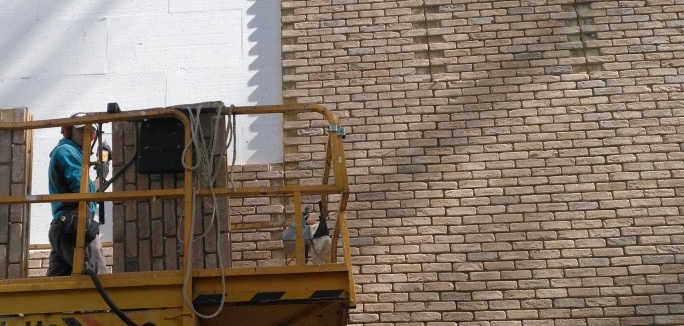
\includegraphics[width=8cm]{pic/Intro.png}
\end{figure}

\section{Introduction}
Soucieux de nous insérer dans la mode actuelle, nous avons souhaité construire des murs. Formation l'oblige, ces murs seront numériques, graphiques même. Si les ouvriers et les entreprises doivent payer chaque brique nouvellement ajoutée, chaque pouce supplémentaire de mur, ce n'est pas le cas pour nous autres, informaticiens. Nous proposons ici, en effet, de générer l'image d'un mur de taille arbitraire à partir d'un échantillon rudimentaire. 
Dans l'ordre, nous décrivons l'algorithme, nous précisons certains choix fait lors de l'implantation, nous exhibons nos résultats, nous discuttons des limitations de cette approche, et enfin nous envisageons un ensemble d'améliorations possibles.

\section{Description de l'algorithme}

Nous basons notre travail sur un article d'Alexei A. Efros et William T. Freeman \cite{efros2001image}, dans lequel est décrit un algorithme simple de génération de textures à base de tuiles. L'algorithme se décrit grossièrement comme :

\begin{itemize}
    \item[1.] Recouvrir la surface à générer de tuiles de même tailles, tirées aléatoirement de la texture échantillon;
    \item[2.] Prendre toutes ces tuiles plus larges que nécessaire pour avoir une marge se superposant avec les tuiles voisines (voir figure \ref{fig:tile});
    \item[3.] Faire la jonction entre deux tuiles voisines en découpant dans les marges selon un chemin de poids minimal, de sorte à minimiser les aberrations lors du collage.
\end{itemize}

\begin{figure}
    \centering
    \scalebox{1.2}{%LaTeX with PSTricks extensions
%%Creator: inkscape 0.92.1
%%Please note this file requires PSTricks extensions
\psset{xunit=.5pt,yunit=.5pt,runit=.5pt}
\begin{pspicture}(322.51340851,224.23202395)
{
\newrgbcolor{curcolor}{0 0 0}
\pscustom[linestyle=none,fillstyle=solid,fillcolor=curcolor,opacity=0]
{
\newpath
\moveto(31.25669291,192.97533766)
\lineto(161.25668811,192.97533766)
\lineto(161.25668811,62.97534246)
\lineto(31.25669291,62.97534246)
\closepath
}
}
{
\newrgbcolor{curcolor}{0.94117647 0 0}
\pscustom[linewidth=2.51338591,linecolor=curcolor]
{
\newpath
\moveto(31.25669291,192.97533766)
\lineto(161.25668811,192.97533766)
\lineto(161.25668811,62.97534246)
\lineto(31.25669291,62.97534246)
\closepath
}
}
{
\newrgbcolor{curcolor}{0 0 0}
\pscustom[linestyle=none,fillstyle=solid,fillcolor=curcolor,opacity=0]
{
\newpath
\moveto(161.25670253,192.97533766)
\lineto(291.25669772,192.97533766)
\lineto(291.25669772,62.97534246)
\lineto(161.25670253,62.97534246)
\closepath
}
}
{
\newrgbcolor{curcolor}{0 0.12156863 0.77254903}
\pscustom[linewidth=2.51338591,linecolor=curcolor]
{
\newpath
\moveto(161.25670253,192.97533766)
\lineto(291.25669772,192.97533766)
\lineto(291.25669772,62.97534246)
\lineto(161.25670253,62.97534246)
\closepath
}
}
{
\newrgbcolor{curcolor}{0 0 0}
\pscustom[linestyle=none,fillstyle=solid,fillcolor=curcolor,opacity=0]
{
\newpath
\moveto(1.25669291,222.97533766)
\lineto(191.25668811,222.97533766)
\lineto(191.25668811,32.97534246)
\lineto(1.25669291,32.97534246)
\closepath
}
}
{
\newrgbcolor{curcolor}{0.96078432 0 0.63529414}
\pscustom[linewidth=2.51338568,linecolor=curcolor,linestyle=dashed,dash=2.65999994 2.65999994]
{
\newpath
\moveto(1.25669291,222.97533766)
\lineto(191.25668811,222.97533766)
\lineto(191.25668811,32.97534246)
\lineto(1.25669291,32.97534246)
\closepath
}
}
{
\newrgbcolor{curcolor}{0 0.11764706 0.71764708}
\pscustom[linestyle=none,fillstyle=solid,fillcolor=curcolor,opacity=0]
{
\newpath
\moveto(131.25671694,222.97533766)
\lineto(321.25671214,222.97533766)
\lineto(321.25671214,32.97534246)
\lineto(131.25671694,32.97534246)
\closepath
}
}
{
\newrgbcolor{curcolor}{0.08235294 0.46666667 0.30980393}
\pscustom[linewidth=2.51338568,linecolor=curcolor,linestyle=dashed,dash=2.65999997 2.65999997]
{
\newpath
\moveto(131.25671694,222.97533766)
\lineto(321.25671214,222.97533766)
\lineto(321.25671214,32.97534246)
\lineto(131.25671694,32.97534246)
\closepath
}
}
{
\newrgbcolor{curcolor}{0 0 0}
\pscustom[linestyle=none,fillstyle=solid,fillcolor=curcolor,opacity=0.38423648]
{
\newpath
\moveto(131.25668811,222.97533766)
\lineto(191.25668811,222.97533766)
\lineto(191.25668811,32.97534246)
\lineto(131.25668811,32.97534246)
\closepath
}
}
{
\newrgbcolor{curcolor}{0.58039218 0 0}
\pscustom[linestyle=none,fillstyle=solid,fillcolor=curcolor,opacity=0.24630545]
{
\newpath
\moveto(31.25669291,192.97527999)
\lineto(161.25668811,192.97527999)
\lineto(161.25668811,192.97527999)
\lineto(161.25668811,62.97528479)
\lineto(161.25668811,62.97528479)
\lineto(31.25669291,62.97528479)
\lineto(31.25669291,62.97528479)
\lineto(31.25669291,192.97527999)
\lineto(31.25669291,192.97527999)
\closepath
}
}
{
\newrgbcolor{curcolor}{0.10196079 0 0.49803922}
\pscustom[linestyle=none,fillstyle=solid,fillcolor=curcolor,opacity=0.2315271]
{
\newpath
\moveto(161.25670253,192.97533766)
\lineto(291.25669772,192.97533766)
\lineto(291.25669772,192.97533766)
\lineto(291.25669772,62.97534246)
\lineto(291.25669772,62.97534246)
\lineto(161.25670253,62.97534246)
\lineto(161.25670253,62.97534246)
\lineto(161.25670253,192.97533766)
\lineto(161.25670253,192.97533766)
\closepath
}
}
{
\newrgbcolor{curcolor}{0.92156863 0.79607844 0}
\pscustom[linewidth=2.13543306,linecolor=curcolor]
{
\newpath
\moveto(166.25668913,222.97533103)
\curveto(154.02096,207.92166174)(144.29028661,190.54653103)(139.49969386,171.6635956)
\curveto(138.42752504,163.60590741)(145.5507515,157.5947956)(153.13223055,157.2676019)
\curveto(161.54241638,156.33659087)(170.27436472,154.63723969)(176.65803591,148.67987276)
\curveto(183.3505285,142.19579087)(182.98408819,127.89137513)(173.22795591,124.56860347)
\curveto(166.38743811,125.54568694)(158.99213858,122.92658772)(158.01592441,115.02635465)
\curveto(156.24895748,108.24682709)(154.99605543,99.92045229)(148.00418646,96.45768694)
\curveto(140.89117228,88.88744442)(143.26525606,76.64529009)(150.54908598,70.10160505)
\curveto(155.77606299,62.96045229)(166.2470778,64.02004284)(171.26887181,57.00331213)
\curveto(175.77146835,51.2987578)(176.20968189,42.57984127)(182.63029417,38.46268851)
\curveto(190.24187717,39.84652473)(185.61750425,29.46495623)(191.25669165,32.97530583)
}
}
{
\newrgbcolor{curcolor}{0 0 0}
\pscustom[linestyle=none,fillstyle=solid,fillcolor=curcolor]
{
\newpath
\moveto(91.38169622,14.09375491)
\lineto(91.38169622,12.42969249)
\curveto(90.85044624,12.92448413)(90.28273794,13.29427578)(89.67857131,13.53906744)
\curveto(89.079613,13.78385909)(88.4415922,13.90625492)(87.76450891,13.90625492)
\curveto(86.43117564,13.90625492)(85.41034236,13.49740077)(84.70200907,12.67969248)
\curveto(83.99367577,11.86719252)(83.63950912,10.69010925)(83.63950912,9.14844267)
\curveto(83.63950912,7.61198441)(83.99367577,6.43490114)(84.70200907,5.61719285)
\curveto(85.41034236,4.80469289)(86.43117564,4.39844292)(87.76450891,4.39844292)
\curveto(88.4415922,4.39844292)(89.079613,4.52083874)(89.67857131,4.7656304)
\curveto(90.28273794,5.01042205)(90.85044624,5.3802137)(91.38169622,5.87500534)
\lineto(91.38169622,4.22656792)
\curveto(90.82961291,3.85156794)(90.24367544,3.57031796)(89.62388381,3.38281797)
\curveto(89.00930051,3.19531798)(88.35825888,3.10156798)(87.67075891,3.10156798)
\curveto(85.905134,3.10156798)(84.51450908,3.64063046)(83.49888413,4.7187554)
\curveto(82.48325918,5.80208868)(81.97544671,7.2786511)(81.97544671,9.14844267)
\curveto(81.97544671,11.02344257)(82.48325918,12.50000499)(83.49888413,13.57812993)
\curveto(84.51450908,14.66146321)(85.905134,15.20312985)(87.67075891,15.20312985)
\curveto(88.36867554,15.20312985)(89.02492551,15.10937985)(89.63950881,14.92187986)
\curveto(90.25930044,14.73958821)(90.84002958,14.46354655)(91.38169622,14.09375491)
\closepath
}
}
{
\newrgbcolor{curcolor}{0 0 0}
\pscustom[linestyle=none,fillstyle=solid,fillcolor=curcolor]
{
\newpath
\moveto(101.04575784,8.60938019)
\lineto(101.04575784,3.32813047)
\lineto(99.60825791,3.32813047)
\lineto(99.60825791,8.5625052)
\curveto(99.60825791,9.39063015)(99.44679959,10.01042179)(99.12388294,10.4218801)
\curveto(98.80096629,10.83333841)(98.31659131,11.03906757)(97.67075801,11.03906757)
\curveto(96.89471639,11.03906757)(96.28273725,10.79167175)(95.83482061,10.29688011)
\curveto(95.38690397,9.80208846)(95.16294564,9.12760933)(95.16294564,8.27344271)
\lineto(95.16294564,3.32813047)
\lineto(93.71763322,3.32813047)
\lineto(93.71763322,15.48437983)
\lineto(95.16294564,15.48437983)
\lineto(95.16294564,10.71875508)
\curveto(95.50669563,11.24479672)(95.91034144,11.63802587)(96.37388308,11.89844252)
\curveto(96.84263306,12.15885917)(97.38169553,12.2890675)(97.9910705,12.2890675)
\curveto(98.99627878,12.2890675)(99.7566954,11.97656752)(100.27232038,11.35156755)
\curveto(100.78794535,10.73177592)(101.04575784,9.81771346)(101.04575784,8.60938019)
\closepath
}
}
{
\newrgbcolor{curcolor}{0 0 0}
\pscustom[linestyle=none,fillstyle=solid,fillcolor=curcolor]
{
\newpath
\moveto(111.41294472,8.06250522)
\lineto(111.41294472,7.35938026)
\lineto(104.80357007,7.35938026)
\curveto(104.86607007,6.36979698)(105.16294505,5.61458868)(105.69419502,5.09375538)
\curveto(106.23065333,4.57813041)(106.97544496,4.32031792)(107.92856991,4.32031792)
\curveto(108.48065321,4.32031792)(109.01450735,4.38802625)(109.53013232,4.52344291)
\curveto(110.05096563,4.65885957)(110.5665906,4.86198456)(111.07700724,5.13281788)
\lineto(111.07700724,3.77344295)
\curveto(110.56138227,3.55469296)(110.03273646,3.3880263)(109.49106982,3.27344297)
\curveto(108.94940319,3.15885965)(108.39992405,3.10156798)(107.84263241,3.10156798)
\curveto(106.44679915,3.10156798)(105.34002838,3.50781796)(104.52232009,4.32031792)
\curveto(103.70982013,5.13281788)(103.30357015,6.23177615)(103.30357015,7.61719275)
\curveto(103.30357015,9.04948434)(103.6889868,10.18490094)(104.45982009,11.02344257)
\curveto(105.23586171,11.86719252)(106.28013249,12.2890675)(107.59263242,12.2890675)
\curveto(108.7697157,12.2890675)(109.69940315,11.90885919)(110.38169478,11.14844256)
\curveto(111.06919474,10.39323427)(111.41294472,9.36458849)(111.41294472,8.06250522)
\closepath
\moveto(109.9754448,8.4843802)
\curveto(109.96502813,9.27083849)(109.74367398,9.89844263)(109.31138233,10.3671926)
\curveto(108.88429902,10.83594258)(108.31659072,11.07031756)(107.60825742,11.07031756)
\curveto(106.80617413,11.07031756)(106.162945,10.84375508)(105.67857002,10.3906301)
\curveto(105.19940338,9.93750512)(104.92336173,9.29948432)(104.85044507,8.4765677)
\closepath
}
}
{
\newrgbcolor{curcolor}{0 0 0}
\pscustom[linestyle=none,fillstyle=solid,fillcolor=curcolor]
{
\newpath
\moveto(120.58481796,10.3984426)
\curveto(120.94419294,11.0442759)(121.37388042,11.52083837)(121.87388039,11.82813003)
\curveto(122.37388036,12.13542168)(122.962422,12.2890675)(123.6395053,12.2890675)
\curveto(124.55096358,12.2890675)(125.25408854,11.96875502)(125.74888019,11.32813005)
\curveto(126.24367183,10.69271342)(126.49106765,9.78646347)(126.49106765,8.60938019)
\lineto(126.49106765,3.32813047)
\lineto(125.04575522,3.32813047)
\lineto(125.04575522,8.5625052)
\curveto(125.04575522,9.40104682)(124.89731773,10.02344262)(124.60044275,10.4296926)
\curveto(124.30356776,10.83594258)(123.85044278,11.03906757)(123.24106782,11.03906757)
\curveto(122.49627619,11.03906757)(121.90773455,10.79167175)(121.47544291,10.29688011)
\curveto(121.04315127,9.80208846)(120.82700544,9.12760933)(120.82700544,8.27344271)
\lineto(120.82700544,3.32813047)
\lineto(119.38169302,3.32813047)
\lineto(119.38169302,8.5625052)
\curveto(119.38169302,9.40625515)(119.23325553,10.02865095)(118.93638054,10.4296926)
\curveto(118.63950556,10.83594258)(118.18117225,11.03906757)(117.56138062,11.03906757)
\curveto(116.82700565,11.03906757)(116.24367235,10.78906758)(115.81138071,10.28906761)
\curveto(115.37908906,9.79427597)(115.16294324,9.122401)(115.16294324,8.27344271)
\lineto(115.16294324,3.32813047)
\lineto(113.71763082,3.32813047)
\lineto(113.71763082,12.07813001)
\lineto(115.16294324,12.07813001)
\lineto(115.16294324,10.71875508)
\curveto(115.49106822,11.25521339)(115.88429737,11.6510467)(116.34263068,11.90625502)
\curveto(116.80096399,12.16146334)(117.34523479,12.2890675)(117.97544309,12.2890675)
\curveto(118.61085973,12.2890675)(119.1499222,12.12760918)(119.59263051,11.80469253)
\curveto(120.04054715,11.48177588)(120.3712763,11.0130259)(120.58481796,10.3984426)
\closepath
}
}
{
\newrgbcolor{curcolor}{0 0 0}
\pscustom[linestyle=none,fillstyle=solid,fillcolor=curcolor]
{
\newpath
\moveto(129.36606663,12.07813001)
\lineto(130.80356656,12.07813001)
\lineto(130.80356656,3.32813047)
\lineto(129.36606663,3.32813047)
\closepath
\moveto(129.36606663,15.48437983)
\lineto(130.80356656,15.48437983)
\lineto(130.80356656,13.66406743)
\lineto(129.36606663,13.66406743)
\closepath
}
}
{
\newrgbcolor{curcolor}{0 0 0}
\pscustom[linestyle=none,fillstyle=solid,fillcolor=curcolor]
{
\newpath
\moveto(141.07700351,8.60938019)
\lineto(141.07700351,3.32813047)
\lineto(139.63950359,3.32813047)
\lineto(139.63950359,8.5625052)
\curveto(139.63950359,9.39063015)(139.47804526,10.01042179)(139.15512861,10.4218801)
\curveto(138.83221196,10.83333841)(138.34783699,11.03906757)(137.70200369,11.03906757)
\curveto(136.92596206,11.03906757)(136.31398293,10.79167175)(135.86606628,10.29688011)
\curveto(135.41814964,9.80208846)(135.19419132,9.12760933)(135.19419132,8.27344271)
\lineto(135.19419132,3.32813047)
\lineto(133.7488789,3.32813047)
\lineto(133.7488789,12.07813001)
\lineto(135.19419132,12.07813001)
\lineto(135.19419132,10.71875508)
\curveto(135.5379413,11.24479672)(135.94158711,11.63802587)(136.40512876,11.89844252)
\curveto(136.87387873,12.15885917)(137.4129412,12.2890675)(138.02231617,12.2890675)
\curveto(139.02752445,12.2890675)(139.78794108,11.97656752)(140.30356605,11.35156755)
\curveto(140.81919102,10.73177592)(141.07700351,9.81771346)(141.07700351,8.60938019)
\closepath
}
}
{
\newrgbcolor{curcolor}{0 0 0}
\pscustom[linestyle=none,fillstyle=solid,fillcolor=curcolor]
{
\newpath
\moveto(154.81137523,10.75000508)
\lineto(154.81137523,15.48437983)
\lineto(156.24887515,15.48437983)
\lineto(156.24887515,3.32813047)
\lineto(154.81137523,3.32813047)
\lineto(154.81137523,4.6406304)
\curveto(154.50929191,4.1197971)(154.12647943,3.73177628)(153.66293779,3.47656796)
\curveto(153.20460448,3.22656798)(152.65252117,3.10156798)(152.00668787,3.10156798)
\curveto(150.94939626,3.10156798)(150.08741714,3.52344296)(149.42075051,4.36719292)
\curveto(148.75929221,5.21094287)(148.42856306,6.32031781)(148.42856306,7.69531774)
\curveto(148.42856306,9.07031767)(148.75929221,10.17969261)(149.42075051,11.02344257)
\curveto(150.08741714,11.86719252)(150.94939626,12.2890675)(152.00668787,12.2890675)
\curveto(152.65252117,12.2890675)(153.20460448,12.16146334)(153.66293779,11.90625502)
\curveto(154.12647943,11.65625503)(154.50929191,11.27083839)(154.81137523,10.75000508)
\closepath
\moveto(149.91293798,7.69531774)
\curveto(149.91293798,6.63802613)(150.12908381,5.80729701)(150.56137545,5.20313037)
\curveto(150.99887543,4.60417207)(151.59783373,4.30469292)(152.35825035,4.30469292)
\curveto(153.11866698,4.30469292)(153.71762528,4.60417207)(154.15512526,5.20313037)
\curveto(154.59262524,5.80729701)(154.81137523,6.63802613)(154.81137523,7.69531774)
\curveto(154.81137523,8.75260935)(154.59262524,9.58073431)(154.15512526,10.17969261)
\curveto(153.71762528,10.78385925)(153.11866698,11.08594256)(152.35825035,11.08594256)
\curveto(151.59783373,11.08594256)(150.99887543,10.78385925)(150.56137545,10.17969261)
\curveto(150.12908381,9.58073431)(149.91293798,8.75260935)(149.91293798,7.69531774)
\closepath
}
}
{
\newrgbcolor{curcolor}{0 0 0}
\pscustom[linestyle=none,fillstyle=solid,fillcolor=curcolor]
{
\newpath
\moveto(166.69419244,8.06250522)
\lineto(166.69419244,7.35938026)
\lineto(160.08481779,7.35938026)
\curveto(160.14731778,6.36979698)(160.44419277,5.61458868)(160.97544274,5.09375538)
\curveto(161.51190105,4.57813041)(162.25669267,4.32031792)(163.20981762,4.32031792)
\curveto(163.76190093,4.32031792)(164.29575507,4.38802625)(164.81138004,4.52344291)
\curveto(165.33221335,4.65885957)(165.84783832,4.86198456)(166.35825496,5.13281788)
\lineto(166.35825496,3.77344295)
\curveto(165.84262999,3.55469296)(165.31398418,3.3880263)(164.77231754,3.27344297)
\curveto(164.2306509,3.15885965)(163.68117177,3.10156798)(163.12388013,3.10156798)
\curveto(161.72804687,3.10156798)(160.62127609,3.50781796)(159.8035678,4.32031792)
\curveto(158.99106785,5.13281788)(158.58481787,6.23177615)(158.58481787,7.61719275)
\curveto(158.58481787,9.04948434)(158.97023451,10.18490094)(159.74106781,11.02344257)
\curveto(160.51710943,11.86719252)(161.56138021,12.2890675)(162.87388014,12.2890675)
\curveto(164.05096341,12.2890675)(164.98065086,11.90885919)(165.66294249,11.14844256)
\curveto(166.35044246,10.39323427)(166.69419244,9.36458849)(166.69419244,8.06250522)
\closepath
\moveto(165.25669252,8.4843802)
\curveto(165.24627585,9.27083849)(165.0249217,9.89844263)(164.59263005,10.3671926)
\curveto(164.16554674,10.83594258)(163.59783844,11.07031756)(162.88950514,11.07031756)
\curveto(162.08742185,11.07031756)(161.44419272,10.84375508)(160.95981774,10.3906301)
\curveto(160.4806511,9.93750512)(160.20460945,9.29948432)(160.13169279,8.4765677)
\closepath
}
}
{
\newrgbcolor{curcolor}{0 0 0}
\pscustom[linestyle=none,fillstyle=solid,fillcolor=curcolor]
{
\newpath
\moveto(179.90512907,10.75000508)
\lineto(179.90512907,15.48437983)
\lineto(181.34262899,15.48437983)
\lineto(181.34262899,3.32813047)
\lineto(179.90512907,3.32813047)
\lineto(179.90512907,4.6406304)
\curveto(179.60304575,4.1197971)(179.22023327,3.73177628)(178.75669163,3.47656796)
\curveto(178.29835832,3.22656798)(177.74627502,3.10156798)(177.10044172,3.10156798)
\curveto(176.04315011,3.10156798)(175.18117099,3.52344296)(174.51450435,4.36719292)
\curveto(173.85304606,5.21094287)(173.52231691,6.32031781)(173.52231691,7.69531774)
\curveto(173.52231691,9.07031767)(173.85304606,10.17969261)(174.51450435,11.02344257)
\curveto(175.18117099,11.86719252)(176.04315011,12.2890675)(177.10044172,12.2890675)
\curveto(177.74627502,12.2890675)(178.29835832,12.16146334)(178.75669163,11.90625502)
\curveto(179.22023327,11.65625503)(179.60304575,11.27083839)(179.90512907,10.75000508)
\closepath
\moveto(175.00669183,7.69531774)
\curveto(175.00669183,6.63802613)(175.22283765,5.80729701)(175.65512929,5.20313037)
\curveto(176.09262927,4.60417207)(176.69158757,4.30469292)(177.4520042,4.30469292)
\curveto(178.21242083,4.30469292)(178.81137913,4.60417207)(179.2488791,5.20313037)
\curveto(179.68637908,5.80729701)(179.90512907,6.63802613)(179.90512907,7.69531774)
\curveto(179.90512907,8.75260935)(179.68637908,9.58073431)(179.2488791,10.17969261)
\curveto(178.81137913,10.78385925)(178.21242083,11.08594256)(177.4520042,11.08594256)
\curveto(176.69158757,11.08594256)(176.09262927,10.78385925)(175.65512929,10.17969261)
\curveto(175.22283765,9.58073431)(175.00669183,8.75260935)(175.00669183,7.69531774)
\closepath
}
}
{
\newrgbcolor{curcolor}{0 0 0}
\pscustom[linestyle=none,fillstyle=solid,fillcolor=curcolor]
{
\newpath
\moveto(191.78793908,8.06250522)
\lineto(191.78793908,7.35938026)
\lineto(185.17856442,7.35938026)
\curveto(185.24106442,6.36979698)(185.53793941,5.61458868)(186.06918938,5.09375538)
\curveto(186.60564768,4.57813041)(187.35043931,4.32031792)(188.30356426,4.32031792)
\curveto(188.85564756,4.32031792)(189.3895017,4.38802625)(189.90512668,4.52344291)
\curveto(190.42595998,4.65885957)(190.94158495,4.86198456)(191.45200159,5.13281788)
\lineto(191.45200159,3.77344295)
\curveto(190.93637662,3.55469296)(190.40773082,3.3880263)(189.86606418,3.27344297)
\curveto(189.32439754,3.15885965)(188.7749184,3.10156798)(188.21762676,3.10156798)
\curveto(186.8217935,3.10156798)(185.71502273,3.50781796)(184.89731444,4.32031792)
\curveto(184.08481448,5.13281788)(183.6785645,6.23177615)(183.6785645,7.61719275)
\curveto(183.6785645,9.04948434)(184.06398115,10.18490094)(184.83481444,11.02344257)
\curveto(185.61085607,11.86719252)(186.65512685,12.2890675)(187.96762678,12.2890675)
\curveto(189.14471005,12.2890675)(190.0743975,11.90885919)(190.75668913,11.14844256)
\curveto(191.44418909,10.39323427)(191.78793908,9.36458849)(191.78793908,8.06250522)
\closepath
\moveto(190.35043915,8.4843802)
\curveto(190.34002249,9.27083849)(190.11866833,9.89844263)(189.68637669,10.3671926)
\curveto(189.25929338,10.83594258)(188.69158507,11.07031756)(187.98325178,11.07031756)
\curveto(187.18116849,11.07031756)(186.53793935,10.84375508)(186.05356438,10.3906301)
\curveto(185.57439774,9.93750512)(185.29835608,9.29948432)(185.22543942,8.4765677)
\closepath
\moveto(188.96762672,16.1250048)
\lineto(190.52231414,16.1250048)
\lineto(187.97543928,13.18750495)
\lineto(186.78012684,13.18750495)
\closepath
}
}
{
\newrgbcolor{curcolor}{0 0 0}
\pscustom[linestyle=none,fillstyle=solid,fillcolor=curcolor]
{
\newpath
\moveto(200.44418914,11.74219253)
\lineto(200.44418914,10.3984426)
\curveto(200.03793916,10.62240092)(199.62908502,10.78906758)(199.2176267,10.89844257)
\curveto(198.81137672,11.0130259)(198.39991841,11.07031756)(197.98325177,11.07031756)
\curveto(197.05096015,11.07031756)(196.32700186,10.77344258)(195.81137688,10.17969261)
\curveto(195.29575191,9.59115098)(195.03793942,8.76302602)(195.03793942,7.69531774)
\curveto(195.03793942,6.62760947)(195.29575191,5.79688034)(195.81137688,5.20313037)
\curveto(196.32700186,4.61458874)(197.05096015,4.32031792)(197.98325177,4.32031792)
\curveto(198.39991841,4.32031792)(198.81137672,4.37500542)(199.2176267,4.48438041)
\curveto(199.62908502,4.59896374)(200.03793916,4.76823456)(200.44418914,4.99219288)
\lineto(200.44418914,3.66406795)
\curveto(200.04314749,3.47656796)(199.62648085,3.33594297)(199.1941892,3.24219298)
\curveto(198.76710589,3.14844298)(198.31137675,3.10156798)(197.82700178,3.10156798)
\curveto(196.50929351,3.10156798)(195.46241857,3.51563046)(194.68637694,4.34375542)
\curveto(193.91033532,5.17188037)(193.5223145,6.28906782)(193.5223145,7.69531774)
\curveto(193.5223145,9.122401)(193.91293948,10.24479677)(194.69418944,11.06250507)
\curveto(195.48064773,11.88021336)(196.55616851,12.2890675)(197.92075177,12.2890675)
\curveto(198.36346008,12.2890675)(198.79575173,12.2421925)(199.2176267,12.14844251)
\curveto(199.63950168,12.05990085)(200.04835583,11.92448419)(200.44418914,11.74219253)
\closepath
}
}
{
\newrgbcolor{curcolor}{0 0 0}
\pscustom[linestyle=none,fillstyle=solid,fillcolor=curcolor]
{
\newpath
\moveto(206.35043785,11.07031756)
\curveto(205.57960456,11.07031756)(204.97022959,10.76823425)(204.52231295,10.16406761)
\curveto(204.0743963,9.56510931)(203.85043798,8.74219269)(203.85043798,7.69531774)
\curveto(203.85043798,6.6484428)(204.07179214,5.82292201)(204.51450045,5.21875537)
\curveto(204.96241709,4.61979707)(205.57439622,4.32031792)(206.35043785,4.32031792)
\curveto(207.11606281,4.32031792)(207.72283361,4.62240124)(208.17075025,5.22656787)
\curveto(208.6186669,5.83073451)(208.84262522,6.65365113)(208.84262522,7.69531774)
\curveto(208.84262522,8.73177602)(208.6186669,9.55208848)(208.17075025,10.15625511)
\curveto(207.72283361,10.76563008)(207.11606281,11.07031756)(206.35043785,11.07031756)
\closepath
\moveto(206.35043785,12.2890675)
\curveto(207.60043778,12.2890675)(208.58220857,11.88281752)(209.2957502,11.07031756)
\curveto(210.00929182,10.25781761)(210.36606264,9.13281767)(210.36606264,7.69531774)
\curveto(210.36606264,6.26302615)(210.00929182,5.13802621)(209.2957502,4.32031792)
\curveto(208.58220857,3.50781796)(207.60043778,3.10156798)(206.35043785,3.10156798)
\curveto(205.09522958,3.10156798)(204.11085463,3.50781796)(203.39731301,4.32031792)
\curveto(202.68897971,5.13802621)(202.33481306,6.26302615)(202.33481306,7.69531774)
\curveto(202.33481306,9.13281767)(202.68897971,10.25781761)(203.39731301,11.07031756)
\curveto(204.11085463,11.88281752)(205.09522958,12.2890675)(206.35043785,12.2890675)
\closepath
}
}
{
\newrgbcolor{curcolor}{0 0 0}
\pscustom[linestyle=none,fillstyle=solid,fillcolor=curcolor]
{
\newpath
\moveto(212.59262457,6.78125529)
\lineto(212.59262457,12.07813001)
\lineto(214.0301245,12.07813001)
\lineto(214.0301245,6.83594279)
\curveto(214.0301245,6.00781783)(214.19158282,5.38542203)(214.51449947,4.96875539)
\curveto(214.83741612,4.55729707)(215.3217911,4.35156792)(215.9676244,4.35156792)
\curveto(216.74366602,4.35156792)(217.35564516,4.59896374)(217.8035618,5.09375538)
\curveto(218.25668678,5.58854702)(218.48324927,6.26302615)(218.48324927,7.11719277)
\lineto(218.48324927,12.07813001)
\lineto(219.92074919,12.07813001)
\lineto(219.92074919,3.32813047)
\lineto(218.48324927,3.32813047)
\lineto(218.48324927,4.6718804)
\curveto(218.13429095,4.14063043)(217.72804097,3.74479712)(217.26449933,3.48438046)
\curveto(216.80616602,3.22917214)(216.27231188,3.10156798)(215.66293691,3.10156798)
\curveto(214.65772863,3.10156798)(213.89470784,3.41406797)(213.37387453,4.03906793)
\curveto(212.85304123,4.6640679)(212.59262457,5.57813035)(212.59262457,6.78125529)
\closepath
\moveto(216.20981188,12.2890675)
\closepath
}
}
{
\newrgbcolor{curcolor}{0 0 0}
\pscustom[linestyle=none,fillstyle=solid,fillcolor=curcolor]
{
\newpath
\moveto(224.2879418,4.6406304)
\lineto(224.2879418,0.00000565)
\lineto(222.84262938,0.00000565)
\lineto(222.84262938,12.07813001)
\lineto(224.2879418,12.07813001)
\lineto(224.2879418,10.75000508)
\curveto(224.59002512,11.27083839)(224.97023343,11.65625503)(225.42856674,11.90625502)
\curveto(225.89210838,12.16146334)(226.44419169,12.2890675)(227.08481665,12.2890675)
\curveto(228.1473166,12.2890675)(229.00929572,11.86719252)(229.67075402,11.02344257)
\curveto(230.33742065,10.17969261)(230.67075396,9.07031767)(230.67075396,7.69531774)
\curveto(230.67075396,6.32031781)(230.33742065,5.21094287)(229.67075402,4.36719292)
\curveto(229.00929572,3.52344296)(228.1473166,3.10156798)(227.08481665,3.10156798)
\curveto(226.44419169,3.10156798)(225.89210838,3.22656798)(225.42856674,3.47656796)
\curveto(224.97023343,3.73177628)(224.59002512,4.1197971)(224.2879418,4.6406304)
\closepath
\moveto(229.17856654,7.69531774)
\curveto(229.17856654,8.75260935)(228.95981655,9.58073431)(228.52231658,10.17969261)
\curveto(228.09002493,10.78385925)(227.4936708,11.08594256)(226.73325417,11.08594256)
\curveto(225.97283754,11.08594256)(225.37387924,10.78385925)(224.93637927,10.17969261)
\curveto(224.50408762,9.58073431)(224.2879418,8.75260935)(224.2879418,7.69531774)
\curveto(224.2879418,6.63802613)(224.50408762,5.80729701)(224.93637927,5.20313037)
\curveto(225.37387924,4.60417207)(225.97283754,4.30469292)(226.73325417,4.30469292)
\curveto(227.4936708,4.30469292)(228.09002493,4.60417207)(228.52231658,5.20313037)
\curveto(228.95981655,5.80729701)(229.17856654,6.63802613)(229.17856654,7.69531774)
\closepath
}
}
{
\newrgbcolor{curcolor}{0 0 0}
\pscustom[linestyle=none,fillstyle=solid,fillcolor=curcolor]
{
\newpath
\moveto(240.53793187,8.06250522)
\lineto(240.53793187,7.35938026)
\lineto(233.92855722,7.35938026)
\curveto(233.99105721,6.36979698)(234.2879322,5.61458868)(234.81918217,5.09375538)
\curveto(235.35564047,4.57813041)(236.1004321,4.32031792)(237.05355705,4.32031792)
\curveto(237.60564036,4.32031792)(238.13949449,4.38802625)(238.65511947,4.52344291)
\curveto(239.17595277,4.65885957)(239.69157775,4.86198456)(240.20199439,5.13281788)
\lineto(240.20199439,3.77344295)
\curveto(239.68636941,3.55469296)(239.15772361,3.3880263)(238.61605697,3.27344297)
\curveto(238.07439033,3.15885965)(237.52491119,3.10156798)(236.96761956,3.10156798)
\curveto(235.5717863,3.10156798)(234.46501552,3.50781796)(233.64730723,4.32031792)
\curveto(232.83480727,5.13281788)(232.42855729,6.23177615)(232.42855729,7.61719275)
\curveto(232.42855729,9.04948434)(232.81397394,10.18490094)(233.58480723,11.02344257)
\curveto(234.36084886,11.86719252)(235.40511964,12.2890675)(236.71761957,12.2890675)
\curveto(237.89470284,12.2890675)(238.82439029,11.90885919)(239.50668192,11.14844256)
\curveto(240.19418189,10.39323427)(240.53793187,9.36458849)(240.53793187,8.06250522)
\closepath
\moveto(239.10043194,8.4843802)
\curveto(239.09001528,9.27083849)(238.86866112,9.89844263)(238.43636948,10.3671926)
\curveto(238.00928617,10.83594258)(237.44157786,11.07031756)(236.73324457,11.07031756)
\curveto(235.93116128,11.07031756)(235.28793214,10.84375508)(234.80355717,10.3906301)
\curveto(234.32439053,9.93750512)(234.04834888,9.29948432)(233.97543221,8.4765677)
\closepath
}
}
{
\newrgbcolor{curcolor}{0.24705882 0.07843138 0}
\pscustom[linestyle=none,fillstyle=solid,fillcolor=curcolor]
{
\newpath
\moveto(46.10438184,133.65239781)
\lineto(56.79383487,133.65239781)
\lineto(56.79383487,132.21359573)
\lineto(52.30815783,132.21359573)
\lineto(52.30815783,121.01633021)
\lineto(50.59005889,121.01633021)
\lineto(50.59005889,132.21359573)
\lineto(46.10438184,132.21359573)
\closepath
}
}
{
\newrgbcolor{curcolor}{0.24705882 0.07843138 0}
\pscustom[linestyle=none,fillstyle=solid,fillcolor=curcolor]
{
\newpath
\moveto(55.5835483,124.7572156)
\lineto(55.5835483,130.49549679)
\lineto(57.14083995,130.49549679)
\lineto(57.14083995,124.81646039)
\curveto(57.14083995,123.91932498)(57.31575314,123.24506283)(57.66557953,122.79367395)
\curveto(58.01540591,122.34792742)(58.54014549,122.12505416)(59.23979826,122.12505416)
\curveto(60.08051006,122.12505416)(60.74348748,122.39306631)(61.22873054,122.92909061)
\curveto(61.71961595,123.46511491)(61.96505865,124.19580067)(61.96505865,125.12114788)
\lineto(61.96505865,130.49549679)
\lineto(63.52235031,130.49549679)
\lineto(63.52235031,121.01633021)
\lineto(61.96505865,121.01633021)
\lineto(61.96505865,122.47205937)
\curveto(61.58702046,121.89653854)(61.1469163,121.4677191)(60.64474617,121.18560105)
\curveto(60.14821839,120.90912535)(59.56987638,120.77088751)(58.90972014,120.77088751)
\curveto(57.82074446,120.77088751)(56.99413856,121.10942917)(56.42990246,121.7865125)
\curveto(55.86566635,122.46359583)(55.5835483,123.45383019)(55.5835483,124.7572156)
\closepath
\moveto(59.50216805,130.72401242)
\closepath
}
}
{
\newrgbcolor{curcolor}{0.24705882 0.07843138 0}
\pscustom[linestyle=none,fillstyle=solid,fillcolor=curcolor]
{
\newpath
\moveto(66.74695955,130.49549679)
\lineto(68.30425121,130.49549679)
\lineto(68.30425121,121.01633021)
\lineto(66.74695955,121.01633021)
\closepath
\moveto(66.74695955,134.18560093)
\lineto(68.30425121,134.18560093)
\lineto(68.30425121,132.21359573)
\lineto(66.74695955,132.21359573)
\closepath
}
}
{
\newrgbcolor{curcolor}{0.24705882 0.07843138 0}
\pscustom[linestyle=none,fillstyle=solid,fillcolor=curcolor]
{
\newpath
\moveto(71.55425126,134.18560093)
\lineto(73.11154291,134.18560093)
\lineto(73.11154291,121.01633021)
\lineto(71.55425126,121.01633021)
\closepath
}
}
{
\newrgbcolor{curcolor}{0.24705882 0.07843138 0}
\pscustom[linestyle=none,fillstyle=solid,fillcolor=curcolor]
{
\newpath
\moveto(84.46961581,126.14523642)
\lineto(84.46961581,125.38351767)
\lineto(77.30945962,125.38351767)
\curveto(77.37716796,124.31146907)(77.69878254,123.49332672)(78.27430337,122.92909061)
\curveto(78.85546655,122.37049687)(79.66232419,122.0912)(80.69487626,122.0912)
\curveto(81.29296653,122.0912)(81.87130854,122.16455069)(82.42990229,122.31125208)
\curveto(82.99413839,122.45795346)(83.55273214,122.67800555)(84.10568352,122.97140832)
\lineto(84.10568352,121.49875208)
\curveto(83.54708978,121.26177292)(82.97439013,121.08121737)(82.38758458,120.95708542)
\curveto(81.80077903,120.83295348)(81.20550994,120.77088751)(80.6017773,120.77088751)
\curveto(79.08962454,120.77088751)(77.89062281,121.21099167)(77.00477213,122.0912)
\curveto(76.1245638,122.97140832)(75.68445964,124.1619465)(75.68445964,125.66281455)
\curveto(75.68445964,127.21446384)(76.10199436,128.44449855)(76.93706379,129.35291868)
\curveto(77.77777559,130.26698117)(78.90906898,130.72401242)(80.33094397,130.72401242)
\curveto(81.60611757,130.72401242)(82.61327902,130.31212006)(83.35242832,129.48833534)
\curveto(84.09721998,128.67019299)(84.46961581,127.55582668)(84.46961581,126.14523642)
\closepath
\moveto(82.91232416,126.60226766)
\curveto(82.90103943,127.45426418)(82.66123909,128.13416869)(82.19292312,128.64198118)
\curveto(81.73024951,129.14979368)(81.11523216,129.40369993)(80.34787105,129.40369993)
\curveto(79.47894745,129.40369993)(78.78211586,129.15825722)(78.25737628,128.66737181)
\curveto(77.73827906,128.1764864)(77.43923393,127.48529717)(77.36024087,126.59380412)
\closepath
}
}
{
\newrgbcolor{curcolor}{0.24705882 0.07843138 0}
\pscustom[linestyle=none,fillstyle=solid,fillcolor=curcolor]
{
\newpath
\moveto(96.83485038,131.96815303)
\lineto(94.51583998,125.67974163)
\lineto(99.16232432,125.67974163)
\closepath
\moveto(95.87000664,133.65239781)
\lineto(97.80815766,133.65239781)
\lineto(102.62391283,121.01633021)
\lineto(100.84656909,121.01633021)
\lineto(99.69552744,124.25786664)
\lineto(93.99956395,124.25786664)
\lineto(92.84852229,121.01633021)
\lineto(91.04578793,121.01633021)
\closepath
}
}
{
\newrgbcolor{curcolor}{0 0 0.27450982}
\pscustom[linestyle=none,fillstyle=solid,fillcolor=curcolor]
{
\newpath
\moveto(215.85059094,133.65239781)
\lineto(226.54004396,133.65239781)
\lineto(226.54004396,132.21359573)
\lineto(222.05436692,132.21359573)
\lineto(222.05436692,121.01633021)
\lineto(220.33626798,121.01633021)
\lineto(220.33626798,132.21359573)
\lineto(215.85059094,132.21359573)
\closepath
}
}
{
\newrgbcolor{curcolor}{0 0 0.27450982}
\pscustom[linestyle=none,fillstyle=solid,fillcolor=curcolor]
{
\newpath
\moveto(225.32975739,124.7572156)
\lineto(225.32975739,130.49549679)
\lineto(226.88704904,130.49549679)
\lineto(226.88704904,124.81646039)
\curveto(226.88704904,123.91932498)(227.06196223,123.24506283)(227.41178862,122.79367395)
\curveto(227.761615,122.34792742)(228.28635458,122.12505416)(228.98600735,122.12505416)
\curveto(229.82671915,122.12505416)(230.48969658,122.39306631)(230.97493963,122.92909061)
\curveto(231.46582504,123.46511491)(231.71126775,124.19580067)(231.71126775,125.12114788)
\lineto(231.71126775,130.49549679)
\lineto(233.2685594,130.49549679)
\lineto(233.2685594,121.01633021)
\lineto(231.71126775,121.01633021)
\lineto(231.71126775,122.47205937)
\curveto(231.33322956,121.89653854)(230.89312539,121.4677191)(230.39095526,121.18560105)
\curveto(229.89442749,120.90912535)(229.31608548,120.77088751)(228.65592923,120.77088751)
\curveto(227.56695355,120.77088751)(226.74034765,121.10942917)(226.17611155,121.7865125)
\curveto(225.61187544,122.46359583)(225.32975739,123.45383019)(225.32975739,124.7572156)
\closepath
\moveto(229.24837714,130.72401242)
\closepath
}
}
{
\newrgbcolor{curcolor}{0 0 0.27450982}
\pscustom[linestyle=none,fillstyle=solid,fillcolor=curcolor]
{
\newpath
\moveto(236.49316865,130.49549679)
\lineto(238.0504603,130.49549679)
\lineto(238.0504603,121.01633021)
\lineto(236.49316865,121.01633021)
\closepath
\moveto(236.49316865,134.18560093)
\lineto(238.0504603,134.18560093)
\lineto(238.0504603,132.21359573)
\lineto(236.49316865,132.21359573)
\closepath
}
}
{
\newrgbcolor{curcolor}{0 0 0.27450982}
\pscustom[linestyle=none,fillstyle=solid,fillcolor=curcolor]
{
\newpath
\moveto(241.30046035,134.18560093)
\lineto(242.857752,134.18560093)
\lineto(242.857752,121.01633021)
\lineto(241.30046035,121.01633021)
\closepath
}
}
{
\newrgbcolor{curcolor}{0 0 0.27450982}
\pscustom[linestyle=none,fillstyle=solid,fillcolor=curcolor]
{
\newpath
\moveto(254.2158249,126.14523642)
\lineto(254.2158249,125.38351767)
\lineto(247.05566872,125.38351767)
\curveto(247.12337705,124.31146907)(247.44499163,123.49332672)(248.02051246,122.92909061)
\curveto(248.60167565,122.37049687)(249.40853328,122.0912)(250.44108535,122.0912)
\curveto(251.03917562,122.0912)(251.61751763,122.16455069)(252.17611138,122.31125208)
\curveto(252.74034748,122.45795346)(253.29894123,122.67800555)(253.85189261,122.97140832)
\lineto(253.85189261,121.49875208)
\curveto(253.29329887,121.26177292)(252.72059922,121.08121737)(252.13379367,120.95708542)
\curveto(251.54698812,120.83295348)(250.95171903,120.77088751)(250.34798639,120.77088751)
\curveto(248.83583363,120.77088751)(247.63683191,121.21099167)(246.75098122,122.0912)
\curveto(245.87077289,122.97140832)(245.43066873,124.1619465)(245.43066873,125.66281455)
\curveto(245.43066873,127.21446384)(245.84820345,128.44449855)(246.68327289,129.35291868)
\curveto(247.52398468,130.26698117)(248.65527808,130.72401242)(250.07715306,130.72401242)
\curveto(251.35232666,130.72401242)(252.35948811,130.31212006)(253.09863741,129.48833534)
\curveto(253.84342907,128.67019299)(254.2158249,127.55582668)(254.2158249,126.14523642)
\closepath
\moveto(252.65853325,126.60226766)
\curveto(252.64724853,127.45426418)(252.40744818,128.13416869)(251.93913221,128.64198118)
\curveto(251.47645861,129.14979368)(250.86144125,129.40369993)(250.09408015,129.40369993)
\curveto(249.22515654,129.40369993)(248.52832495,129.15825722)(248.00358537,128.66737181)
\curveto(247.48448816,128.1764864)(247.18544302,127.48529717)(247.10644997,126.59380412)
\closepath
}
}
{
\newrgbcolor{curcolor}{0 0 0.27450982}
\pscustom[linestyle=none,fillstyle=solid,fillcolor=curcolor]
{
\newpath
\moveto(264.06738762,127.05083537)
\lineto(264.06738762,122.42127812)
\lineto(266.80957509,122.42127812)
\curveto(267.72927995,122.42127812)(268.40918445,122.61029721)(268.84928862,122.9883354)
\curveto(269.29503514,123.37201596)(269.5179084,123.95600033)(269.5179084,124.74028851)
\curveto(269.5179084,125.53021906)(269.29503514,126.11138225)(268.84928862,126.48377808)
\curveto(268.40918445,126.86181627)(267.72927995,127.05083537)(266.80957509,127.05083537)
\closepath
\moveto(264.06738762,132.2474499)
\lineto(264.06738762,128.43885619)
\lineto(266.59798655,128.43885619)
\curveto(267.43305599,128.43885619)(268.05371571,128.59402112)(268.4599657,128.90435097)
\curveto(268.87185806,129.22032319)(269.07780424,129.69992388)(269.07780424,130.34315304)
\curveto(269.07780424,130.98073984)(268.87185806,131.45751935)(268.4599657,131.77349157)
\curveto(268.05371571,132.08946379)(267.43305599,132.2474499)(266.59798655,132.2474499)
\closepath
\moveto(262.35775222,133.65239781)
\lineto(266.72493968,133.65239781)
\curveto(268.02832508,133.65239781)(269.03266535,133.38156447)(269.73796048,132.83989781)
\curveto(270.44325562,132.29823115)(270.79590318,131.52804887)(270.79590318,130.52935096)
\curveto(270.79590318,129.75634749)(270.61534763,129.14133014)(270.25423652,128.68429889)
\curveto(269.89312541,128.22726765)(269.36274347,127.94232841)(268.6630907,127.82948119)
\curveto(269.5038025,127.64892564)(270.1554952,127.27088745)(270.61816881,126.69536662)
\curveto(271.08648478,126.12548815)(271.32064276,125.41172948)(271.32064276,124.5540906)
\curveto(271.32064276,123.42561839)(270.93696221,122.5538736)(270.1696011,121.93885625)
\curveto(269.40224,121.32383889)(268.31044314,121.01633021)(266.89421051,121.01633021)
\lineto(262.35775222,121.01633021)
\closepath
}
}
\end{pspicture}
}
	\caption{Deux tuiles adjacentes, leur franges en pointillés, et la zone d'intersection en gris. Le chemin jaune correspond à un chemin de poids minimal sur la superposition des tuiles et des franges.\label{fig:tile}}
\end{figure}

Un point important à noter, et qui rends l'algorithme efficace, est que, dans la mesure où chaque pixel ne peut avoir que 8 voisins, et que les poids associés pendant l'étape 3. sont positifs, la recherche de plus court chemin peut être réalisée en temps linéaire en le nombre de pixels à considérer par un parcours en profondeur.

Le pseudo-algorithme cache, bien sûr, de nombreux détails d'implantation, que nous discuterons principalement en section \ref{sec:tech}. Néanmoins, on peut dors et déjà relever les difficultés majeures auxquelles nous aurons à faire face.
Pour le point 1., il faut sélectionner de "bonnes" tuiles, de sorte à ne pas avoir une tuile majoritairement bleue juxtaposée à une tuile majoritairement jaune. Nous avons besoin de discriminer les tuiles et de juger de la qualité de la juxtaposition brute (ie. sans traitement supplémentaire). Pour le point 3., il faut choisir et spécifier la méthode de pondération utilisée. 

Malgré ces difficultés, l'algorithme reste intuitif et relativement simple, et promet de bonnes performances à la génération. Procédons à l'implantation.

% Algorithme en trois étapes:
% 1. Recouvrir la surface souhaitée de tuiles aléatoires de l'image d'origine, en incluant des franges "de collage"
% % TODO Schéma
% 2. Tracer le chemin de poids minimal sur la frange entre deux tuiles % TODO: Trouver une meilleur formualtion
% 3. Couper et recoller les tuiles selon ce chemin

%Difficultés:
%- En 1., il fqut sélectionner de "bonnes" tuiles. Des tuiles cohérentes qui permetterons un collage minimisant les abérrations
%- En 2., il faut spécifier la distance utilisée. 
%- En 2., il faut aussi imposer quelle tuile prends la précédence dans le cas où plusieurs franges se superposent
%

\section{Details techinques d'implantation et choix}

\label{sec:tech}
Le code est fractionné en plusieurs classes pour favoriser sa modularité. La logique de l'application réside dans les classes \texttt{Canvas} et \texttt{Tile}. Le reste correspond majoritairement à des utilitaires de gestion de l'image écrits par nos soins. 

Nous appliquons l'algorithme précédent. La première tuile est sélectionnée aléatoirement, puis les suivantes sont ajoutées dans l'ordre de rastérisation (ligne par ligne, de gauche à droite). La sélection d'une "bonne" tuile se fait vis-à-vis de celles de gauche et du haut. De même, l'étape de découpage se fait systématiquement par rapport à la tuile directement sur la gauche, \emph{puis} par rapport à la tuile supérieure. % TODO dessin ? 

% TODO: Dessin
Dans notre implantation, une \emph{tuile} est un morceau de l'échantillon initial composé du contenu à afficher et de la frange, comme nous l'avons vu sur la figure \ref{fig:tile}. Même si la gestion des franges en devient plus facile, nous ajoutons une difficulté lors du recouvrement et du découpage dans la frange : la frange d'une tuile recouvre maintenant les tuiles de gauche, du haut et du coin supérieur-gauche, comme l'illustre la figure \ref{fig:conflict}. Il faut donc donner une priorité lors des tests de superposition. 

\begin{figure}
    \centering
    \scalebox{1.2}{%LaTeX with PSTricks extensions
%%Creator: inkscape 0.92.4
%%Please note this file requires PSTricks extensions
\psset{xunit=.5pt,yunit=.5pt,runit=.5pt}
\begin{pspicture}(256.41481415,256.41478531)
{
\newrgbcolor{curcolor}{0.32156864 0.72941178 0.72549021}
\pscustom[linestyle=none,fillstyle=solid,fillcolor=curcolor,opacity=0.14903846]
{
\newpath
\moveto(110.63883502,255.77594789)
\lineto(220.63883982,255.77594789)
\lineto(220.63883982,145.77594308)
\lineto(110.63883502,145.77594308)
\closepath
}
}
{
\newrgbcolor{curcolor}{0.32156864 0.4509804 0.72549021}
\pscustom[linewidth=1.27767484,linecolor=curcolor]
{
\newpath
\moveto(110.63883502,255.77594789)
\lineto(220.63883982,255.77594789)
\lineto(220.63883982,145.77594308)
\lineto(110.63883502,145.77594308)
\closepath
}
}
{
\newrgbcolor{curcolor}{0.13333334 0.49411765 0}
\pscustom[linestyle=none,fillstyle=solid,fillcolor=curcolor,opacity=0.14117648]
{
\newpath
\moveto(0.63883742,255.77594789)
\lineto(110.63883502,255.77594789)
\lineto(110.63883502,145.77594308)
\lineto(0.63883742,145.77594308)
\closepath
}
}
{
\newrgbcolor{curcolor}{0.13333334 0.49411765 0}
\pscustom[linewidth=1.27767484,linecolor=curcolor,strokeopacity=0.96634614]
{
\newpath
\moveto(0.63883742,255.77594789)
\lineto(110.63883502,255.77594789)
\lineto(110.63883502,145.77594308)
\lineto(0.63883742,145.77594308)
\closepath
}
}
{
\newrgbcolor{curcolor}{0.17647059 0.07843138 0}
\pscustom[linestyle=none,fillstyle=solid,fillcolor=curcolor,opacity=0.3269234]
{
\newpath
\moveto(0.63883742,145.7759575)
\lineto(110.63882781,145.7759575)
\lineto(110.63882781,35.7759527)
\lineto(0.63883742,35.7759527)
\closepath
}
}
{
\newrgbcolor{curcolor}{0.17647059 0.07843138 0}
\pscustom[linewidth=1.27767473,linecolor=curcolor]
{
\newpath
\moveto(0.63883742,145.7759575)
\lineto(110.63882781,145.7759575)
\lineto(110.63882781,35.7759527)
\lineto(0.63883742,35.7759527)
\closepath
}
}
{
\newrgbcolor{curcolor}{0.92156863 0 0}
\pscustom[linestyle=none,fillstyle=solid,fillcolor=curcolor,opacity=0.13942309]
{
\newpath
\moveto(110.63883502,145.7759575)
\lineto(220.63883261,145.7759575)
\lineto(220.63883261,35.7759599)
\lineto(110.63883502,35.7759599)
\closepath
}
}
{
\newrgbcolor{curcolor}{0.84313726 0 0}
\pscustom[linewidth=1.27767473,linecolor=curcolor]
{
\newpath
\moveto(110.63883502,145.7759575)
\lineto(220.63883261,145.7759575)
\lineto(220.63883261,35.7759599)
\lineto(110.63883502,35.7759599)
\closepath
}
}
{
\newrgbcolor{curcolor}{0.13333334 0.59215689 0}
\pscustom[linestyle=none,fillstyle=solid,fillcolor=curcolor]
{
\newpath
\moveto(75.63883021,180.77597673)
\lineto(110.6388206,180.77597673)
\lineto(110.6388206,145.77600796)
\lineto(75.63883021,145.77600796)
\closepath
}
}
{
\newrgbcolor{curcolor}{0.32156864 0.72941178 0.72549021}
\pscustom[linestyle=none,fillstyle=solid,fillcolor=curcolor,opacity=0.96153843]
{
\newpath
\moveto(110.63883502,180.77597673)
\lineto(220.63883261,180.77597673)
\lineto(220.63883261,145.77600796)
\lineto(110.63883502,145.77600796)
\closepath
}
}
{
\newrgbcolor{curcolor}{0.17647059 0.07843138 0}
\pscustom[linestyle=none,fillstyle=solid,fillcolor=curcolor,opacity=0.86057693]
{
\newpath
\moveto(75.63883021,145.7759575)
\lineto(110.6388206,145.7759575)
\lineto(110.6388206,35.7759599)
\lineto(75.63883021,35.7759599)
\closepath
}
}
{
\newrgbcolor{curcolor}{0.84313726 0 0}
\pscustom[linewidth=1.55196832,linecolor=curcolor,linestyle=dashed,dash=3.28499965 3.28499965]
{
\newpath
\moveto(75.63883021,180.77597673)
\lineto(255.63883021,180.77597673)
\lineto(255.63883021,0.77597673)
\lineto(75.63883021,0.77597673)
\closepath
}
}
\end{pspicture}
}
	\caption{Mise en valeur des zones de conflits suite à l'introduction de la nouvelle tuile (rouge). Les conflits gémérés par les franges des trois autres tuiles déjà installées (vert, bleu, gris) ne sont pas représentés, mais existent en pratique.\label{fig:conflict}}
\end{figure}

% TODO: Dessin
Nous résolvons le problème de la sélection d'une "bonne" tuile en prenant une tuile de poids minimal sur \texttt{N} essais aléatoires. Le poids d'une tuile correspond à la distance sur la norme 2 entre l'ensemble des pixels de la frange de la nouvelle tuile et des anciennes tuiles sur lesquelles celle-ci viendrait se superposer.\texttt{N} est fixé, et vaut 35 dans la plupart de nos expérimentations. 
Cette méthode nous démarque de l'article. Celui-ci propose de prendre une tuile dont la distance sur la frange est en dessous d'un certain seuil. L'introduction de cette notion de seuil ne permet de garantir la terminaison de l'algorithme que presque sûrement. Notre version termine toujours. 



% Utilisation d'un ensemble de classes favorisant la modularité du code.
% 
% % TODO: Schema
% Franges : tout autour de la tuile.
% Pour les difficultés évoquées,
% - On sélectionne la meilleur de X tuiles prises aléatoirement, avec comme mesure la somme des distances (norme 2) sur chaque pixel de superposition entre les tuiles
% - Même distance que ci-dessus
% - On  traite d'abord la frange avec la tuile sur la gauche, puis avec la tuile au dessus.
% 
% Choix:
% Par rapport à l'article, nous ajoutons une étape de coupe horizontale, qui évite l'abérration des pommes. %TODO
% L'article ne spécifie pas le mode de sélection des "bonnes" tuiles.

\section{Resultats}

	De par le fonctionnement de notre algorithme, si nous sommes capables de générer des textures convaincantes de petite taille à partir d'un échantillon donné, alors nous serons capables de générer des textures correctes de plus grande envergure. Nous ne représenterons donc ici que des textures de taille moyenne, en général de l'ordre de $1200\times800$ pixels. 


\subsection{Extension de motifs distingués}
Intéressons-nous à une texture dont les motifs sont définis par leurs contours, telle qu'une texture de grillage ou de lattes de bois. Dans ce cas, l'élement principal de la texture est le trait séparant les différents éléments. Au vu du fonctionnement de l'algorithme, l'etape de découpe devrait permettre de gérer particulièrement bien ces cas, dans la mesure où le trait représentera une forte discontinuité que le chemin minimal cherchera à éviter. 

\begin{figure}%
    \centering
	%\adjincludegraphics[height=5cm,trim={0 0 {.5\width} 0},clip]{example-image-a}
	\subfloat[Échantillon]{{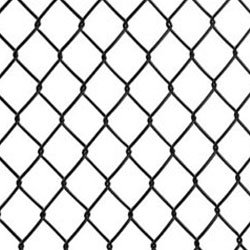
\includegraphics[width=6cm, trim={0 0 0 4.4cm}, clip]{pic/grillage1.png} }}%
    \qquad
    \subfloat[Taille de tuile: 64pxl, Taille de frange: 32pxl]{{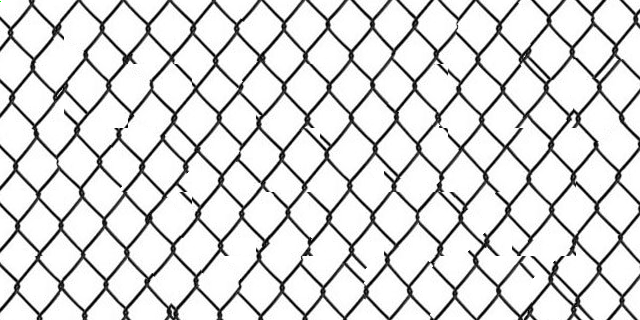
\includegraphics[width=6cm]{pic/grillage1_64_32.png} }}%
    \caption{Génération à partir d'un échantillon distingué}%
    \label{fig:grillage1}%
\end{figure}

\begin{figure}%
    \centering
	\subfloat[Échantillon]{{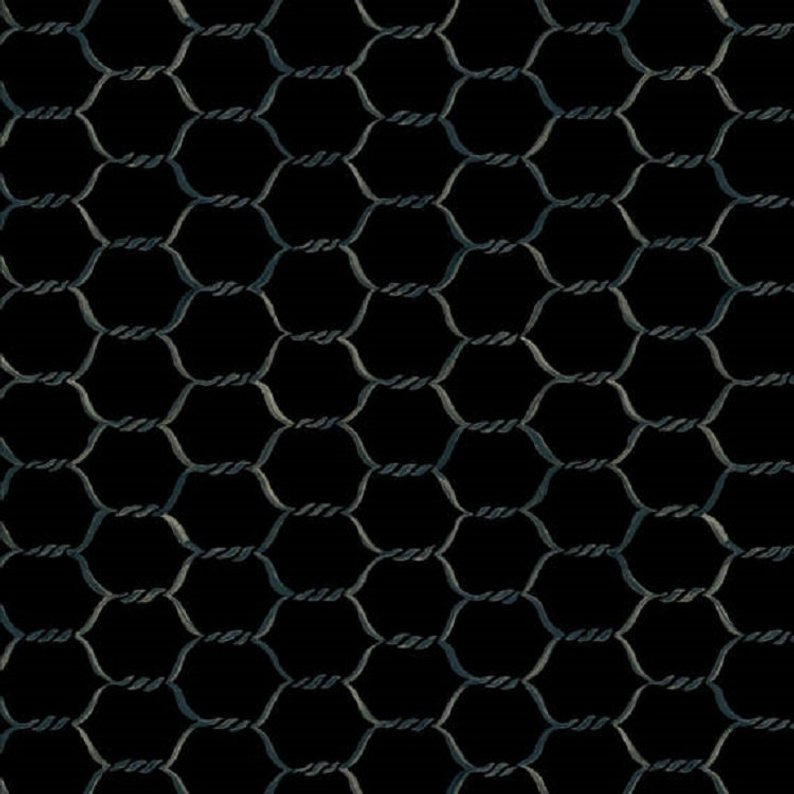
\includegraphics[width=6cm, trim={0 0 0 14cm}, clip]{pic/grillage3.png} }}%
    \qquad
    \subfloat[Taille de tuile: 120pxl, Taille de frange: 50pxl]{{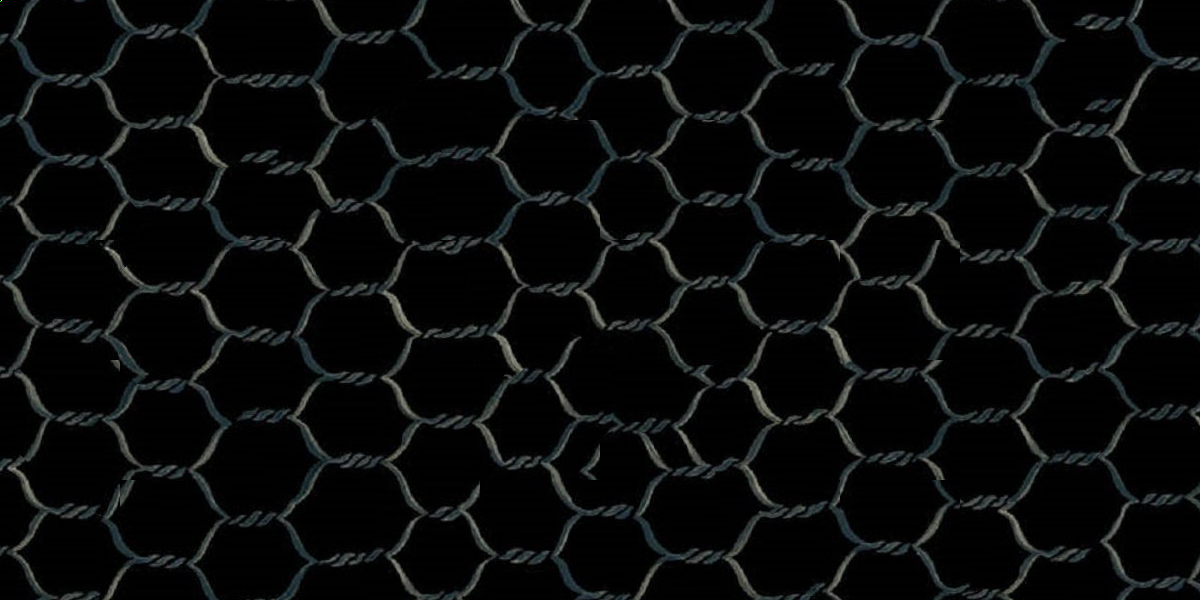
\includegraphics[width=6cm]{pic/grillage3_120_50.png} }}%
    \caption{Autre échantillon de grillage}%
    \label{fig:grillage3}%
\end{figure}
%

On en fait l'expérience en figures \ref{fig:grillage1} et \ref{fig:grillage3}. La génération est relativement bonne, si ce n'est les morceaux de grillages flottant au milieux des cellules. Ces erreurs sont causées par un mauvais choix de tuiles, à cause duquel même une découpe optimale ne pourrais rendre l'image réaliste.




\subsection{Généralisation de motifs déconstruits}

On constate que l'algorithme produit de bons résultats sur les échantillons à très faible granularité, comme la fourrure ou, dans le cas présent, un coup de pinceau. Ce résultat tient au fait que la taille minimale de tuile nécessaire pour capturer l'essence du motif est quasi nulle. Ainsi la texture générée en figure \ref{fig:orange}, a nécessité une taille de tuile de seulement 30 pixels de côté.

\begin{figure}
	\centering
	\subfloat[Échantillon]{{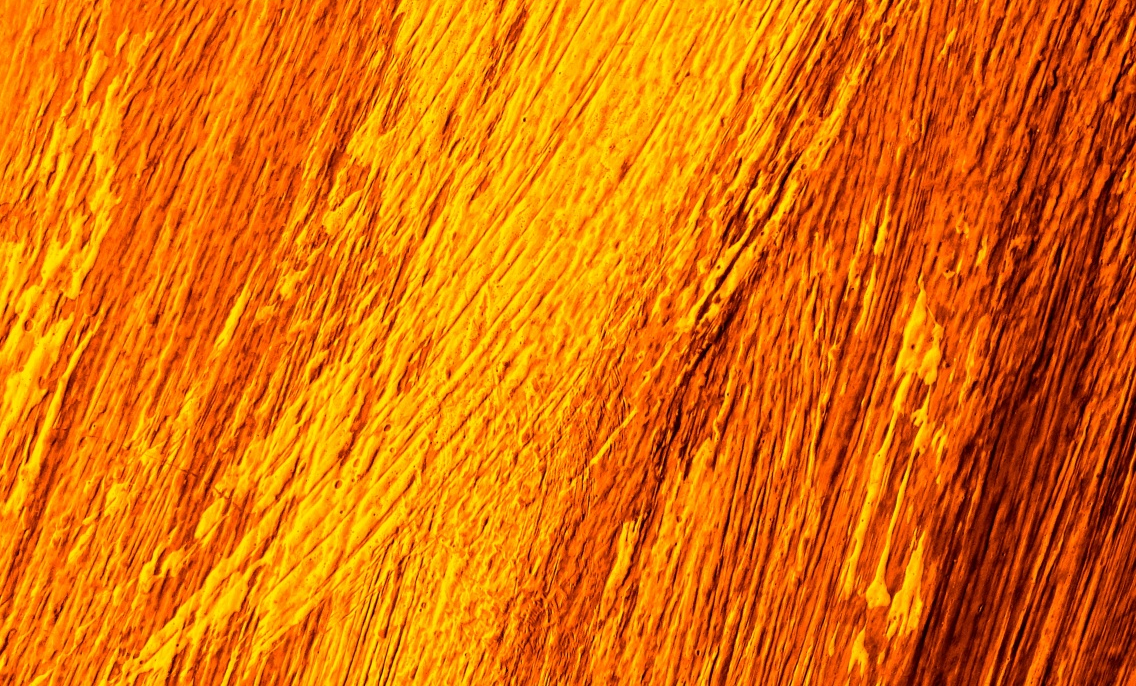
\includegraphics[width=6cm, trim={0 0 0 4.4cm}, clip]{pic/orange_stroke.png} }}
	\qquad
		\subfloat[Taille de tuile: 30pxl, Taille de frange: 10pxl]{{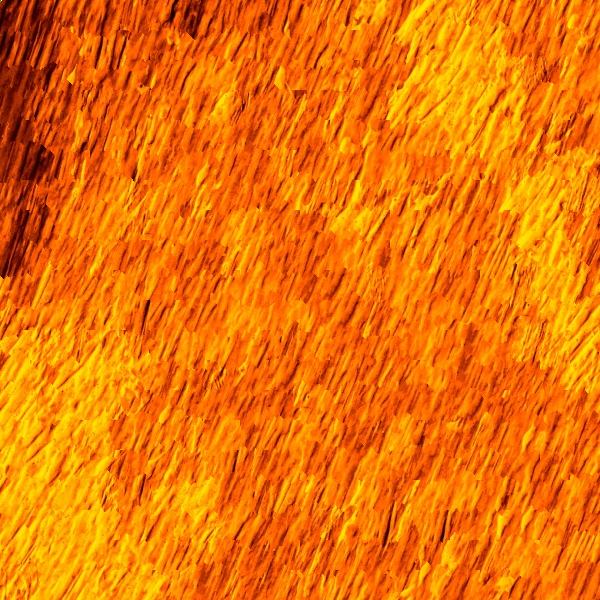
\includegraphics[width=6cm, trim={0, 0, 0, 10.5cm}, clip]{pic/orange_stroke_30_10.png} }}
	\caption{Génération sur un motif faiblement répétitif\label{fig:orange}}
\end{figure}

\subsection{Influence de la taille de tuile et de frange}

Considérons maintenant une structure plus complexe. Nous utilisons toujours des briques, mais celles-ci sont maintenant plus bruitées. L'échantillon est représenté en figure \ref{fig:brick}.

Avec de petites tuiles, comme en figure \ref{fig:brickb}, on n'arrive à capturer que la texture du fond des tuiles, ie. du bruit. Si on augmente progressivement la taille de celles-ci (figure \ref{fig:brickc} et \ref{fig:brickd}), on observe l'apparition des formes des tuiles. Pour être exact, on observe l'apparition du \emph{bord} des briques. 
Malgré un certain nombre d'aberrations, ces figures représentent un résultat qui devient convaincant. Nous verrons en section \ref{sec:prop} des propositions pour améliorer ce résultat.

% TODO: USE grillage1_64_32.png & grillage3_120_50.png

% \documentclass[10pt,a4paper]{article}
% \usepackage[demo]{graphicx}
% \usepackage{subfig}
% \begin{document}
\begin{figure}%
    \centering
	\subfloat[Échantillong]{{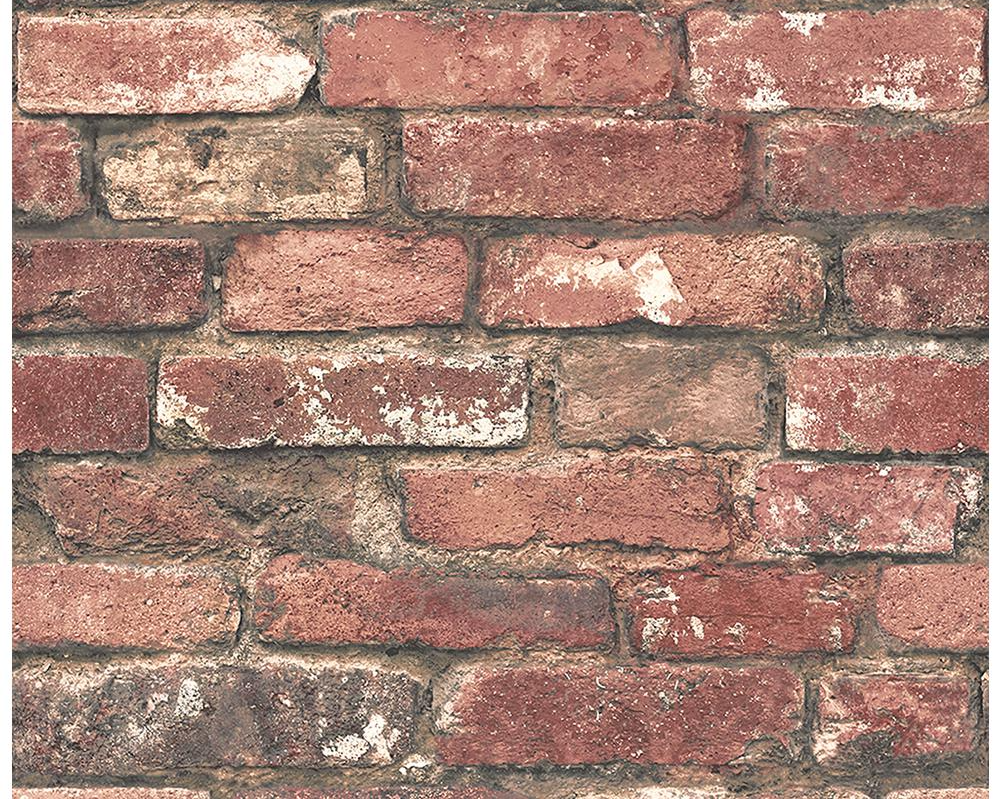
\includegraphics[width=6cm, trim={0 0 0 10.5cm}, clip]{pic/dbrick_cut.png} }}%
    \qquad
    \subfloat[Taille de tuile: 48pxl, Taille de frange: 15pxl\label{fig:brickb}]{{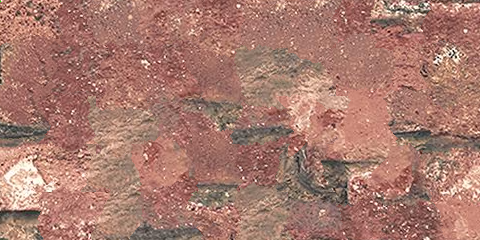
\includegraphics[width=6cm]{pic/dbrick_48_15.png} }}%
    \qquad
    \subfloat[Taille de tuile: 72pxl, Taille de frange: 15pxl\label{fig:brickc}]{{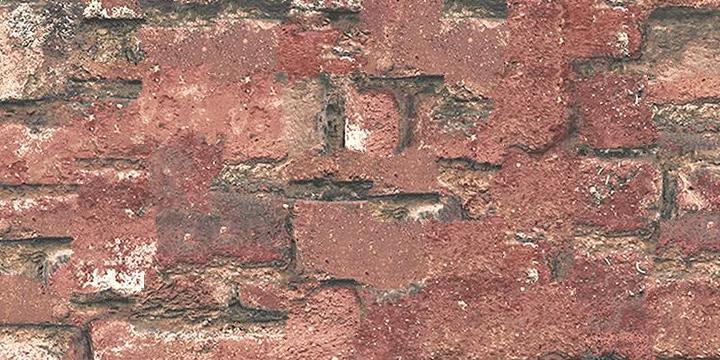
\includegraphics[width=6cm]{pic/dbrick_72_15.png} }}%
    \qquad
    \subfloat[Taille de tuile: 100pxl, Taille de frange: 40pxl\label{fig:brickd}]{{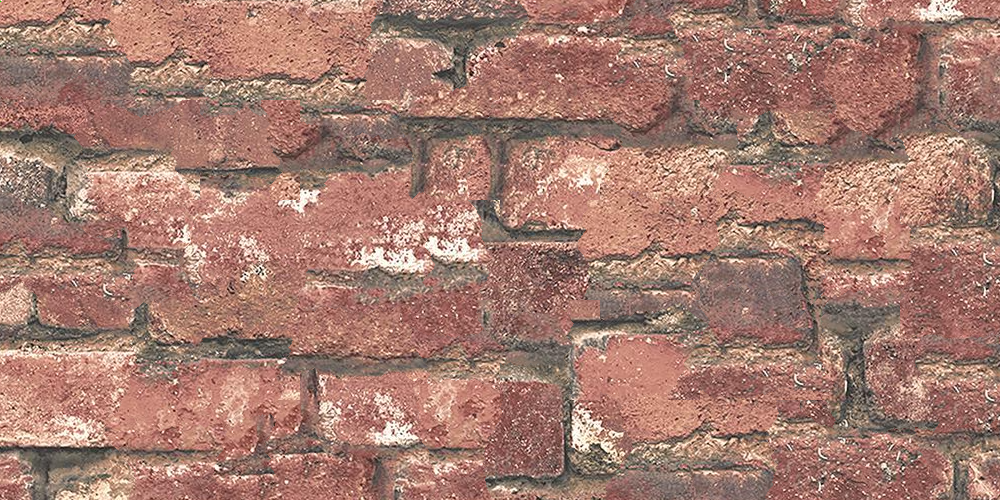
\includegraphics[width=6cm]{pic/dbrick_100_40.png} }}%
    %\qquad
    %\subfloat[TODO]{{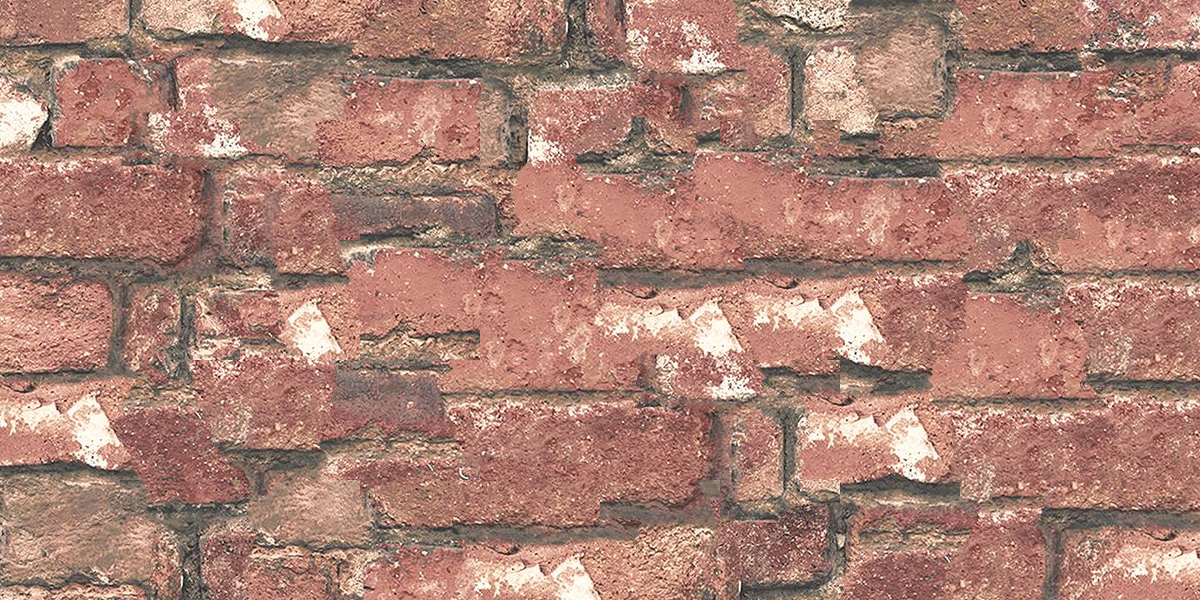
\includegraphics[width=5cm]{pic/dbrick_120_50.png} }}%
    \caption{Évolution de la qualité de l'extension en fonction de la taille de tuile}%
    \label{fig:brick}%
\end{figure}
% \end{document}

% La taille de la tuile et de sa frange sont les seuls paramètres à réellement devoir être ajusté en fonction de la texture. Les franges doivent être suffisament grosses pour intégrer une partie significative du motif (pour avoir des collages propres), mais ne doit pas être trop gros, au risque d'impacter les performances et ajouter du bruit lors du découpage. La tuile doit être assez grosse pour pouvoir intégrer au moins un motif pour minimiser les abérrations.
% 
% 
% L'algo fonctionne remarquablement bien sur les structures très ordonnées et au motif petit.

\section{Limitations}

Tel que décrit, l'algorithme est difficilement parallélisable. La partie de sélection des bonnes tuiles - goulot d'étranglement de l'algorithme - n'est parallélisable qu'avec des méthodes qui ne sont pas raisonnablement généralisables. Étant donné les dépendances lors de la sélection d'une "bonne" tuile, on pourrait imaginer de générer en premier la ligne centrale, puis en parallèle de générer les tuiles au-dessus de cette ligne et en dessous. Mais cette méthode nécessite de changer la logique de génération.

La seconde limitation majeure que nous avons vu ci-dessus vient du choix de la taille de la tuile et de la frange. Ces paramètres vont fortement influer sur la qualité de la texture générée et doivent être choisis avec soin en fonction de l'échantillon. L'algorithme n'est donc pas applicable génériquement sur tout un ensemble de textures. 


%Le code actuel n'est parallèlisable que pour la partie de découpage. Or le réel goulot d'étranglement a lieu sur la partie de sélection des "bonnes" tuiles, qui est peu parallèlisable.
%Possible de paralleliser : Prendre au hasard une ligne centrale puis faire l'expansion des deux côtés en parallèle. Mais difficile à mettre en oeuvre pour un gain faible.
%
%Si la tuile est mal choisie, le coup de ciseau ne fera qu'apporter de nouvelles abérrations.

\section{Améliorations possibles}

\subsection{Performances}

En matière de performance, il faudrait recoder une partie de la classe \texttt{Tuile}, notamment la fonction \texttt{get\_tile}, héritée de \texttt{Picture.cpp}, qui recopie \emph{manuellement} tous les pixels d'une sous-image avant de renvoyer une copie. Cette fonction est lourdement sollicitée lors de l'étape de sélection des "bonnes" tuiles, qui est le goulot d'étranglement du programme. Étant donné que pendant cette étape, aucune modification n'est réalisée, il aurait été souhaitable que la fonction \texttt{get\_tile} se contente de renvoyer une référence constante, et évite de recopier l'objet. 
Nous pensons que cette amélioration pourrait, à elle seule, grandement améliorer les performances à l'exécution. La section en question représentant, après profilage, 71\% du temps total d'exécution pour la génération d'une image de $20\times10$ tuiles. 

\subsection{Qualité}
\label{sec:prop}

Le but de l'étape de découpage est de limiter les aberrations. Celles-ci sont néanmoins inévitables si les tuiles juxtaposées sont mal choisies. La sélection de "bonnes" tuiles est donc le facteur majoritaire déterminant la qualité du résultat produit. Dans l'idéal, un effort important serait placé dans la recherche d'un algorithme plus efficace de sélection des "bonnes" tuiles, pour remplacer notre algorithme trop naïf.

Dans un second temps, on pourrait raisonnablement imaginer une métrique plus complexe pour réaliser le découpage. Cette étape est peu coûteuse et permet de bien mettre en valeur les discontinuités des images, comme dans la figure \ref{fig:grillage3}. Une métrique prenant en compte la morphologie des éléments présents, telle que celles vues en cours, pourraient donc représenter une substantielle amélioration. 

Enfin, on peut automatiser la sélection de la taille des tuiles. Lors de la sélection, le point important est de s'assurer que la tuile est suffisamment grosse pour accueillir un ou plusieurs motifs. Tout repose donc sur la période spatiale des motifs de l'image. La transformée de fourrier est l'outil privilégié pour déterminer ce type de longueur caractéristiques. Il est ainsi probable que l'on puisse déterminer automatiquement une taille correcte pour la tuile simplement à partir de la transformée de fourier de l'image. 

% Choisir une métrique plus intelligente pour la sélection des tuiles et le découpage.
% Pour la sélection, précalculer un ensemble de tuiles similaires, quitte à réduire le nombre de tuiles sélectionnable aléatoirement au début.
% La métrique de sélection doit être rapide à calculer car il s'agit de l'opération limitatrice de l'algo.
% La métrique de découpage peut être plus subtile et peut se permettre d'être plus coûteuse, par exemple en intégrant des élements de morphologie.
% 
% - Selection automatique de la taille des tuiles:
%     . Calculer la transformée de Fourier de l'image pour en déduire la longueur caractéristique des motifs
%     . (Filtrer les longueur parasites, telles que les recouvrement de couleur)
%     . Assigner cette taille à la taille de tuile, et diviser par quatre pour la taille de frange. 
% 

\section{Conclusion}
L'algorithme présenté ici est simple dans sa description. Et malgré son caractère non parallèlisable, il permet de générer une extension de texture avec une faible quantité de calcul. L'algorithme fonctionne avec très peu de paramètres, ce qui en fait un outil d'approximation de texture utilisable par le plus grand nombre. Il permet notamment de respecter les jonctions sur les motifs fortement marqués tels que les grillages ou les briques. On peut lui reprocher la naïveté de son approche, qui le rends difficilement améliorable, mais on peut tout à fait imaginer l'utiliser dans un context de génération "quick and dirty", comme par exemple lors de la prévisualisation d'une scène 3D.

%C'est simple, rapide sur un single thread, peu gourmand en calcul, facilement paramètrable, ready-to-use et efficace pour les textures à motif trés fort;
%mais peu ou pas parallèlisable, et trop naïf lorsque les motifs sont plus étendus ou complexes.
%
%Utilisable dans les logiciels de rendu 3D pour une texturisation rapide (et moche) lors de la visualisation. 

%\begin{figure}[h]
%    \centering
%    \scalebox{.6}{\input{../svg/neurons.tex}}
%    \caption{toto}
%\end{figure}


\bibliographystyle{plain}
\bibliography{report}

\end{document}

